\begingroup %{
\newcommand{\bou}{{\,|\,}}
\newcommand{\boug}{{\,\big|\,}}
\newcommand{\bougg}{{\,\bigg|\,}}
\newcommand{\q}[1]{{\blr{#1}}}
\newcommand{\qg}[1]{{\blrg{#1}}}
\newcommand{\qgg}[1]{{\blrgg{#1}}}
\newcommand{\qggg}[1]{{\blrggg{#1}}}
\newcommand{\qgggg}[1]{{\blrgggg{#1}}}
\newcommand{\qa}[1]{{\blra{#1}}}
\newcommand{\qD}{{\op{D}}}
\newcommand{\qI}{{\op{I}}}
\newcommand{\hqI}{{\what{\op{I}}}}
\newcommand{\opN}{{\op{N}}}
\newcommand{\opL}{{\op{L}}}
\newcommand{\opR}{{\op{R}}}
\newcommand{\grow}{{\op{grow}}}
\newcommand{\code}{{\op{code}}}
\newcommand{\sumw}{{\op{sum}}}
\newcommand{\sym}{{\op{sym}}}
\newcommand{\word}[1]{{|\!\lfloor{#1}\rfloor\!|}}
\newcommand{\sword}[1]{{\{\!\lfloor{#1}\rfloor\!\}}}
\newcommand{\hf}{{\what{f}}}
{\setlength\arraycolsep{2pt}
%
\section{微分方程式と二分木}\label{s1:微分方程式と二分木} %{
\subsection{$q=1$の場合}\label{s2:q=1の場合} %{
	$\plr{f\bou x}\in R\bblr{x}$とし、$x_t\in R\bblr{t,x}$を次の微分方程式の
	解とする。
	\begin{equation*}\begin{split}
		x_t = x + \int_t\plr{f\bou x_t}
	\end{split}\end{equation*}
	$x_t = \blrg{t\plr{f\bou x}\partial_x}_1^*x$とTalor展開できて、
	次のように二分木の成長と対応する。
	\begin{equation*}\begin{split}
		\plr{f\bou x} \xmapsto{\partial_x} \xymatrix@R=2pt@C=2pt{
			\bullet \hen[d]\hen[r] & \partial f \\
			f \\
		} \xmapsto{\partial_x} \xymatrix@R=2pt@C=2pt{
			\bullet \hen[d]\hen[r] & \partial f \\
			\circ \hen[d]\hen[r] & \partial f \\
			f \\
		} + \xymatrix@R=2pt@C=2pt{
			\bullet \hen[d]\hen[r] & \circ \hen[d]\hen[r] 
			& \partial^2 f \\
			f & f \\
		} \quad\text{where } \partial^nf := \plr{\partial^nf\bou x}
	\end{split}\end{equation*}
	したがって、次の対応が成り立つことが予想される。
	\begin{equation*}\begin{split}
		x_t - x \sim \qgg{t\grow}_1^*\bullet
	\end{split}\end{equation*}
%s2:q=1の場合}
\subsection{q-微分方程式}\label{s2:q-微分方程式} %{
	$\plr{f\bou x}\in R_q\bblr{x}$とし、$x_t\in R_q\bblr{t,x}$を次の
	微分方程式の解とする。
	\begin{equation}\label{eq:微分方程式そのゼロ}\begin{split}
		x_t = x + \qI_t\plr{f\bou x_t}
	\end{split}\end{equation}
	$y_t := \plr{f\bou x_t}$とおくと、$x_t = x + \qI_ty_t$となり、
	$y_t$は次のように書ける。
	\begin{equation}\label{eq:微分方程式その一}\begin{split}
		y_t = \plr{f\bou x_t} = \plrg{f\bou x + \qI_ty_t}
		= \sum_{n\in\sizen}\frac{\plr{\qI_ty_t}^n}{n!}\plr{\partial^nf\bou x}
	\end{split}\end{equation}
	$y_t$を二分木の成長に対応させることを考える。

	二分木を自然数の配列に符号化したものを考える。節\ref{s2:二分木の符号化}
	にしたがい、写像$\sumw:\sizen^+\to\sizen$と$\opN:\sizen^+\to\sizen^+$を
	次のように定義し、
	\begin{alignat*}{2}
		\sumw\word{n_1,\dots,n_k} &:= n_1 +\cdots+ n_k
			&&\quad\text{for all } n_1,\dots,n_k\in\sizen \\
		\opN_\sizen w &:= \plr{\sumw\, w} w &&\quad\text{for all } w\in\sizen^+
	\end{alignat*}
	線形射$\grow_\sizen:R_q\sizen^+\to R_q\sizen^+$を次のように定義する。
	\begin{equation*}\begin{split}
		\grow_\sizen\word{n} &:= \word{0,n+1} \quad\text{for all } n\in\sizen \\
		\grow_\sizen m_0 &:= m_0\plr{\grow_\sizen\otimes1 + q^{\opN_\sizen}\otimes\grow_\sizen}
	\end{split}\end{equation*}
	そして、$Y_t\in R_q\sizen^+\bblr{t}$を次のように定義すると、
	\begin{equation}\label{eq:Y_tの定義}\begin{split}
		Y_t := \plr{t\,\grow_\sizen}^*\word{0}
	\end{split}\end{equation}
	$Y_t$は次のように書ける。
	\begin{equation}\label{eq:木の成長その一}\begin{split}
		Y_t &= \sum_{n\in\sizen}\plr{\hqI_t Y_t}^n\word{n}
	\end{split}\end{equation}
	ここで、$\hqI_t$は多重積分を表すとする。
	\begin{equation*}\begin{split}
		\plr{\hqI_t Y_t}^n
		:= \underbrace{\qI_t Y_t\cdots\qI_t Y_t}_{n\text{ times}}
	\end{split}\end{equation*}
	\begin{proof} %{
		節\ref{s2:Leibniz則とKleeneスター}を使う。
		\begin{equation*}\begin{split}
			Y_t	&= \word{0} + \qI_t \plr{t\,\grow_\sizen}^*\grow_\sizen\word{0} \\
			&= \word{0} + \qI_t \plr{t\,\grow_\sizen}^*\word{0,1} \\
			&= \word{0} + \qI_t m_0\plrgg{\plr{t\,\grow_\sizen}^*\otimes1}
				\plrgg{q^{\opN_\sizen}\otimes\plr{t\,\grow_\sizen}^*}
				\plrgg{\word{0}\otimes\word{1}} \\
			&= \word{0} + \qI_t Y_t\plr{t\,\grow_\sizen}^*\word{1} \\
			&= \word{0} + \qI_t Y_t\word{1}
				+ \qI_t Y_t\qI_t Y_t\plr{t\,\grow_\sizen}^*\word{2} \\
			&= \cdots \\
			&= \sum_{n\in\sizen}\plr{\hqI_t Y_t}^n\word{n}
		\end{split}\end{equation*}
	\end{proof} %}
	\eqref{eq:微分方程式その一}と\eqref{eq:木の成長その一}は、
	それぞれ、積分の積と多重積分という違いを除いて似た形になっている。

	$q=0$と$q=1$の時に限り、多重積分は積分の積の形に書き換えることができる。
	\begin{itemize}\setlength{\itemsep}{-1mm} %{
		\item $q=0$の時 \\
		任意の$g_1,\dots,g_k\in R_q\bblr{t}$に対して次の式が成り立つ。
		\begin{equation*}\begin{split}
			\hqI_tg_1\cdots\hqI_tg_k = \plr{\qI_tg_1}\cdots\plr{\qI_tg_k} 
		\end{split}\end{equation*}
		\begin{proof} %{
			直接の計算により、任意の$n_1,\dots,n_k\in\sizen$に対して次の式が
			成り立つことがわかる。
			\begin{equation*}\begin{split}
				\hqI_tt^{n_1}\cdots\hqI_tt^{n_k} = t^{n_1+\cdots+n_k+k}
				= \plr{\qI_tt^{n_1}}\cdots\plr{\qI_t^{n_k}} 
			\end{split}\end{equation*}
		\end{proof} %}
		\item $q=1$の時 \\
		任意の$g\in R_q\bblr{t}$に対して次の式が成り立つ。
		\begin{equation*}\begin{split}
			\plr{\hqI_tg}^n = \frac{\plr{\qI_tg}^n}{n!}
		\end{split}\end{equation*}
		\begin{proof} %{
			ベキ$n$についての帰納法で証明する。$n=1$の時は明らかに命題が成り立つ。
			ある$n\in\sizen_+$以下で命題が成り立つと仮定すると、部分積分により、
			次の式が成り立ち、
			\begin{equation*}\begin{split}
				\plr{\hqI_tg}^{n+1} &= \hqI_tg\plr{\hqI_tg}^n 
				= \plr{\qI_tg}\plr{\hqI_tg}^n 
					- \hqI_t\plr{\qI_tg}g\plr{\hqI_tg}^{n-1} \\
				&= \plr{\qI_tg}\plr{\hqI_tg}^n - n\hqI_tg\plr{\hqI_tg}^n 
				= \plr{\qI_tg}\plr{\hqI_tg}^n - n\plr{\hqI_tg}^{n+1} \\
				&= \frac{\plr{\qI_tg}\plr{\hqI_tg}^n}{n+1}
			\end{split}\end{equation*}
			$n+1$でも命題が成り立つことがわかる。
		\end{proof} %}
	\end{itemize} %}
	したがって、$q=0$と$q=1$の時に限り、次の式が成り立つ。
	\begin{equation*}\begin{split}
		Y_t = \begin{cases}
			\sum_{n\in\sizen}\plr{\qI_tY_t}^n\word{n}, &\text{ if } q = 0 \\
			\sum_{n\in\sizen}\cfrac{\plr{\qI_tY_t}^n}{n!}\word{n}, &\text{ if } q = 1 \\
		\end{cases}
	\end{split}\end{equation*}

	一般の$q$に戻って、任意の$\plr{g\bou x}\in R_q\bblr{x}$に対して、
	代数射$(g)_x:R_q\sizen^+\to R_q\bblr{x}$を次のように定義すると、
	\begin{equation*}\begin{split}
		(g)_x\word{n} := \frac{\q{n}!}{n!}\plr{\partial^ng\bou x}
		\quad\text{for all } n\in\sizen
	\end{split}\end{equation*}
	次の式が成り立つ。
	\begin{equation*}\begin{split}
		(f)_xY_t = \sum_{n\in\sizen}\frac{\q{n}!\plr{\hqI_t(f)_xY_t}^n}{n!}
			\plr{\partial^nf\bou x}
	\end{split}\end{equation*}
	そして、$q=0$と$q=1$の時に限り、多重積分を次のように書き換えることができる。
	\begin{equation*}\begin{split}
		(f)_xY_t = \sum_{n\in\sizen}\frac{\plr{\qI_t(f)_xY_t}^n}{n!}
			\plr{\partial^nf\bou x}
		= \plr{f\bou x + \qI_t(f)_xY_t} \quad\text{at } \left\{\begin{split}
				q &= 0 \\ q &= 1
			\end{split}\right.
	\end{split}\end{equation*}
	この式は\eqref{eq:微分方程式その一}に等しい。このことを命題の形にまとめて
	おく。

	\begin{proposition}[微分方程式と二分木]\label{prop:微分方程式と二分木} %{
		任意の$\plr{f\bou x}\in R_q\bblr{x}$に対して、
		代数射$(f)_x:R_q\sizen^+\to R_q\bblr{x}$を次のように定義し、
		\begin{equation*}\begin{split}
			(f)_x\word{n} := \frac{\q{n}!}{n!}\plr{\partial^nf\bou x}
			\quad\text{for all } n\in\sizen
		\end{split}\end{equation*}
		$Y_t\in R_q\sizen^+\bblr{t}$を次のように定義すると、
		\begin{equation*}\begin{split}
			Y_t := \plr{t\,\grow_\sizen}^*\word{0}
		\end{split}\end{equation*}
		$q=0$または$q=1$の時、次の微分方程式が成り立つ。
		\begin{equation*}\begin{split}
			(f)_xY_t = \plr{f\bou x + \qI_t(f)_xY_t} 
			\quad\text{at } \left\{\begin{split}
				q &= 0 \\ q &= 1
			\end{split}\right.
		\end{split}\end{equation*}
	\end{proposition} %prop:微分方程式と二分木}
	\begin{proof} %{
		上記。
	\end{proof} %}

\begin{note}[保留]\label{note:保留} %{
	\begin{itemize}\setlength{\itemsep}{-1mm} %{
		\item 一般の$q$の場合の多重積分 \\
		$R_q$上のテンソル積$\otimes$を考えると、一般には次の式が成り立つ。
		\begin{equation*}\begin{split}
			\hqI_tf\hqI_tg = \frac{1}{\q{N_t}}m_0\plrg{\q{N_t}\otimes1}\plrg{\qI_tf\otimes\qI_tg}
			\quad\text{for all } f,g\in R_q\bblr{t}
		\end{split}\end{equation*}
		特に、次の式が成り立つ。
		\begin{equation*}\begin{split}
			\hqI_tf\hqI_tf = \frac{1}{2\q{N_t}}m_0
				\plrg{\q{N_t}\otimes1 + 1\otimes\q{N_t}}\plrg{\qI_tf\otimes\qI_tf}
			\quad\text{for all } f\in R_q\bblr{t}
		\end{split}\end{equation*}
		%
		\item 計算の高速化 \\
		最終的には体へ写像してしまうので、非可換な文字列のまま計算するより、
		可換な文字列を計算した方が効率的になる。
		次の可換図を満たす?があれば都合が良いのだが、多分ないだろう\footnote{
			$q=1$の時は通常の微分$\sword{n}^{k+1}\mapsto(k+1)\sword{n}^k\sword{n+1}$
			が?になるが、一般の$q$ではわからない。
		}。
		\begin{equation*}\begin{split}
			\xymatrix{
				R_q\dlr{\sizen} \ar[d]^{\grow_\sizen} \ar[r]^\sym 
				& R_q\blr{\sizen} \ar@{.>}[d]^? \\
				R_q\dlr{\sizen} \ar[r]^\sym & R\blr{\sizen} \\
			}
		\end{split}\end{equation*}
	\end{itemize} %}
\end{note} %note:保留}
\begin{landscape}
	\begin{note}[符号の計算]\label{note:符号の計算} %{
		命題\ref{prop:微分方程式と二分木}を使って微分方程式
		\ref{eq:微分方程式そのゼロ}の解を書いてみる。
		$Y_n:=\grow_\sizen^n\word{0}$とおき、$4$次まで計算すると次のようになる。
		\begin{equation}\label{eq:符号の計算}\begin{split}
			Y_0 &= \word{0} \\
			Y_1 &= \word{0}\word{1} \\
			Y_2 &= \word{0}\word{1}^2 + \word{0}^2\word{2} \\
			Y_3 &= \word{0}\word{1}^3 + (3 + q)\word{0}^2\word{1}\word{2} 
				+ \word{0}^3\word{3}\\
			Y_4 &= \word{0}\word{1}^4 + (6 + 3q + 2q^2)\word{0}^2\word{1}^2\word{2}
				+ (2 + q + q^2)\word{0}^3\word{2}^2
				+ (4 + 2q + q^2)\word{0}^3\word{1}\word{3} + \word{0}^4\word{4}		
		\end{split}\end{equation}
		微分方程式\ref{eq:微分方程式そのゼロ}の解を
		$x_t = \sum_{n\in\sizen}\frac{t^n}{\q{n}!} x_n$とTaylor展開すると、
		$x_{n+1} = f^xY_n$となる。そして、$(f\bou x)=x^2$とすると、
		任意の$n\in\sizen$に対して$(\partial^nf\bou x)$は$\sizen$係数となる。
		初期値$x=1$として$7$次まで計算した結果は次のようになる。
		\begin{equation*}\begin{split}
			x_1 &= 1 \\
			x_2 &= 2 \\
			x_3 &= 5 + q \\
			x_4 &= 14 + 8q + 2q^2 \\
			x_5 &= 42 + 41q + 25q^2 + 11q^3 + q^4 \\
			x_6 &= 132 + 184q + 164q^2 + 132q^3 + 76q^4 + 28q^5 + 4q^6 \\
			x_7 &= 429 + 780q + 893q^2 + 923q^3 + 830q^4 + 606q^5 + 351q^6
				+ 173q^7 + 49q^8 + 6q^9 \\
			x_8 &= 1430 + 3212q + 4450q^2 + 5422q^3 + 5962q^4 + 5838q^5 
				+ 5034q^6 + 3840q^7 + 2558q^8 + 1526q^9 + 736q^{10} + 254q^{11} 
				+ 54q^12 + 4q^{13}
		\end{split}\end{equation*}
		$x_n$は$q=0$でCatalan数$C_n$、$q=1$で階乗$n!$になっていることがわかる。
		図\ref{fig:q-Catalan係数の分布}は、$x_{10}$まで計算して、
		横軸に$n$縦軸に$q^n$の係数をプロットしている。\EOP
	\end{note} %note:符号の計算}
\end{landscape}

	\begin{figure}[htbp] %{
		\begin{center}
			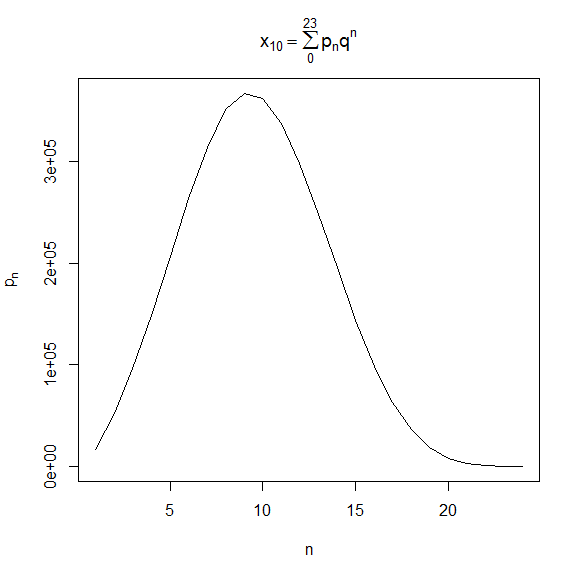
\includegraphics[width=100mm]{fig/x-10.png}
		\end{center}
		\caption{q-Catalan係数の分布}\label{fig:q-Catalan係数の分布}
	\end{figure} %}
%s2:q-微分方程式}
\subsection{Leibniz則とKleeneスター}\label{s2:Leibniz則とKleeneスター} %{
	$R$を可換環、$V=(V,\mu)$を$R_q$上の代数とする。
	\begin{itemize}\setlength{\itemsep}{-1mm} %{
		\item 線形射$\opN:V\to V$はLeibniz則、
		$\opN\mu = \mu\plr{\opN\otimes1 + 1\otimes\opN}$、を満たすとする。
		\item 線形射$\gamma:V\to V$はLeibniz則、
		$\gamma\mu = \mu\plr{\gamma\otimes1 + q^\opN\otimes\gamma}$、を満たし、
		$\opN$と交換関係、
		$\opN\gamma = \gamma\plr{\opN + 1}$
		、を満たすとする。
	\end{itemize} %}
	$\opN$を次数と言うことにすると、$\gamma$は次数を一つ上げる演算となる。

	線形射$\Delta:\cat{Mod}\plr{V}\to\cat{Mod}\plr{V\otimes V}$を次のように
	定義する。
	\begin{equation*}\begin{split}
		\phi\mu := \mu\plr{\Delta\phi} \quad\text{where }\phi\in\cat{Mod}\plr{V}
	\end{split}\end{equation*}
	$\Delta$は常に定義できるとは限らないと思うが、$\opN$と$\gamma$に対しては
	定義できる。そして、$\Delta$が定義できる場合は、次の性質が成り立つ。
	\begin{itemize}\setlength{\itemsep}{-1mm} %{
		\item 余結合的、
		$\plr{\Delta\otimes1}\Delta = \plr{1\otimes\Delta}\Delta$ 、になる。
		\item 写像の合成に対して準同型となる。
		\begin{equation*}\begin{split}
			\Delta\plr{\phi\psi} = \plr{\Delta\phi}\plr{\Delta\psi}
			\quad\text{where }\phi,\psi\in\cat{Mod}\plr{V}
		\end{split}\end{equation*}
	\end{itemize} %}
	したがって、$\Delta$は、余単位射以外、$\cat{Mod}\plr{V}$と双代数をなす。

	$\Delta\gamma^n$は次の式を満たす。
	\begin{equation*}\begin{split}
		\Delta\gamma^n = \sum_{r=0}^n\qbinom{n}{r}
			\plr{\gamma^rq^{\plr{n-r}\opN}\otimes\gamma^{\plr{n-r}\opN}} 
			\quad\text{for all } n\in\sizen
	\end{split}\end{equation*}
	\begin{proof} %{
		$n$についての帰納法で証明される。
		二項係数のPascal三角の公式を使って次の式が得られる。
		\begin{equation*}\begin{split}
			\Delta\gamma^{n+1} &= \plr{\Delta\gamma}
				\sum_{r=0}^n\qbinom{n}{r}\plr{\gamma^rq^{\plr{n-r}\opN}
				\otimes\gamma^{\plr{n-r}\opN}} \\
			&= \sum_{r=0}^n\qbinom{n}{r}\plr{\gamma^{r+1}q^{\plr{n-r}\opN}
				\otimes\gamma^{\plr{n-r}\opN} + q^{\opN}\gamma^rq^{\plr{n-r}\opN}
				\otimes\gamma^{\plr{n+1-r}\opN}} \\
			&= \sum_{r=0}^n\qbinom{n}{r}\plr{\gamma^{r+1}q^{\plr{n-r}\opN}
				\otimes\gamma^{\plr{n-r}\opN} + q^r\gamma^rq^{\plr{n+1-r}\opN}
				\otimes\gamma^{\plr{n+1-r}\opN}} \\
			&= \gamma^{n+1}\otimes1 + q^{\plr{n+1}\opN}\otimes\gamma^{n+1}
				+ \sum_{r=1}^n\plra{\qbinom{n}{r-1} + q^r\qbinom{n}{r}}
				\plr{\gamma^rq^{\plr{n+1-r}\opN}\otimes\gamma^{n+1-r}} \\
			&= \sum_{r=0}^{n+1}\qbinom{n+1}{r}\plr{\gamma^rq^{\plr{n+1-r}\opN}
				\otimes\gamma^{\plr{n+1-r}\opN}}
		\end{split}\end{equation*}
	\end{proof} %}
	この式から次の因子化が得られる。
	\begin{equation*}\begin{split}
		\Delta\gamma^* = \plr{\gamma^*\otimes1}\plr{q^\opN\otimes\gamma}^*
	\end{split}\end{equation*}
	特に、$q=1$の時は、$\gamma^*$は群的な作用素となる。
	一般の$q$でも群的に近い形になっている。特に、作用するテンソル積の
	一項目の次数が$0$の時は、群的に振る舞う。
	\begin{equation*}\begin{split}
		\opN u = 0 \implies \gamma^*\mu\plr{u\otimes v}
		= \mu\plr{\gamma^*\otimes\gamma^*}\plr{u\otimes v}
		\quad\text{for all } u,v\in V
	\end{split}\end{equation*}

	\begin{todo}[Leibniz則とKleeneスター]\label{todo:Leibniz則とKleeneスター} %{
		逆Kleeneスターと積との交換関係を求める。
	\end{todo} %todo:Leibniz則とKleeneスター}
%s2:Leibniz則とKleeneスター}
\subsection{二分木の符号化}\label{s2:二分木の符号化} %{
	線形射$\code_\sizen:R_q\clB_*\to R_q\sizen^+$を二分木の符号化ということ
	にする。
	\begin{equation*}\begin{split}
		\code_\sizen\bullet := \word{0}
		,\quad \code_\sizen\beta := m_0\plr{1\otimes\opR_+}
		\plr{\code_\sizen\otimes\code_\sizen}
	\end{split}\end{equation*}
	線形射$\opN_\sizen:R_q\sizen^+\to R_q\sizen^+$を次のように定義し、
	\begin{equation*}\begin{split}
		\opN_\sizen w = \plr{\sumw_\sizen w}w \quad\text{for all } w\in\sizen^+
	\end{split}\end{equation*}
	線形射$\grow_\sizen:R_q\sizen^+\to R_q\sizen^+$を次のように定義すると、
	\begin{equation*}\begin{split}
		\grow_\sizen\word{n} &:= \word{0,n+1} \quad\text{for all } n\in\sizen \\
		\grow_\sizen m_0 &:= m_0\plr{\grow_\sizen\otimes1 
		+ q^{\opN_\sizen}\otimes\grow_\sizen}
	\end{split}\end{equation*}
	次の交換関係を満たす。
	\begin{enumerate}\setlength{\itemsep}{-1mm} %{
		\item $\opN_\sizen\code_\sizen = \code_\sizen\opN$
		\item $\grow_\sizen\code_\sizen = \code_\sizen\grow$
		\item\label{eq:自然数列の成長その一} $\opR_+\grow_\sizen = \grow_\sizen\opR_+$
		\item\label{eq:自然数列の成長その二} $\opN_\sizen\grow_\sizen = \grow_\sizen\plr{\opN_\sizen + 1}$
	\end{enumerate} %}
	\begin{proof} %{
		項目毎に証明する。
		\begin{enumerate}\setlength{\itemsep}{-1mm} %{
			\item 二分木の次数についての帰納法で証明する。
			次数$0$の時には命題が成り立つ。
			\begin{equation*}\begin{split}
				\code_\sizen\opN\bullet = \code_\sizen0 = 0 
				= \opN_\sizen\word{0} = \opN_\sizen\code_\sizen\bullet
			\end{split}\end{equation*}
			次数$n$以下で命題が成り立つと仮定する。$\beta$と$\code_\sizen,\opN$
			との交換関係から次の式が成り立つ。
			\begin{equation*}\begin{split}
				\code_\sizen\opN\beta 
				= m_0\plr{1\otimes\opR_+}\plr{\code_\sizen\otimes\code_\sizen}
					\plr{\opN\otimes1 + 1\otimes\opN + 1\otimes1} \\
			\end{split}\end{equation*}
			任意の$r,s\le n$に対して、$\clB_r\otimes\clB_s$に作用させると、
			帰納法の仮定から次の式が成り立ち、
			\begin{equation*}\begin{split}
				& \code_\sizen\opN\beta\plr{\clB_r\otimes\clB_s} \\
				&= m_0\plr{1\otimes\opR_+}\plr{\code_\sizen\otimes\code_\sizen}
					\plr{\opN\otimes1 + 1\otimes\opN + 1\otimes1}
					\plr{\clB_r\otimes\clB_s} \\
				&= m_0\plr{1\otimes\opR_+}
					\plr{\opN_\sizen\otimes1 + 1\otimes\opN_\sizen + 1\otimes1}
					\plr{\code_\sizen\otimes\code_\sizen}
					\plr{\clB_r\otimes\clB_s} \\
				&= m_0\plr{\opN_\sizen\otimes1 + 1\otimes\opN_\sizen}
					\plr{1\otimes\opR_+}
					\plr{\code_\sizen\otimes\code_\sizen}
					\plr{\clB_r\otimes\clB_s} \\
				&= \opN_\sizen\code_\sizen\beta\plr{\clB_r\otimes\clB_s} \\
			\end{split}\end{equation*}
			次数が$n+1$でも命題が成り立つことがわかる。
			%
			\item 二分木の次数についての帰納法で証明する。
			次数$0$の時には命題が成り立つ。
			\begin{equation*}\begin{split}
				\code_\sizen\grow\bullet 
				= \code_\sizen\beta\plr{\bullet\otimes\bullet} = \word{0,1}
				= \grow_\sizen\word{0} = \grow_\sizen\code_\sizen\bullet
			\end{split}\end{equation*}
			次数$n$以下で命題が成り立つと仮定する。$\beta$と$\code_\sizen,\grow$
			との交換関係から次の式が成り立つ。
			\begin{equation*}\begin{split}
				\code_\sizen\grow\beta 
				= m_0\plr{1\otimes\opR_+}\plr{\code_\sizen\otimes\code_\sizen}
					\plr{\grow\otimes1 + q^{\opN}\otimes\grow} \\
			\end{split}\end{equation*}
			任意の$r,s\le n$に対して、$\clB_r\otimes\clB_s$に作用させると、
			帰納法の仮定と命題\ref{eq:自然数列の成長その一}から、
			次の式が成り立ち、
			\begin{equation*}\begin{split}
				& \code_\sizen\grow\beta\plr{\clB_r\otimes\clB_s} \\
				&= m_0\plr{1\otimes\opR_+}\plr{\code_\sizen\otimes\code_\sizen}
					\plr{\grow\otimes1 + q^{\opN}\otimes\grow}
					\plr{\clB_r\otimes\clB_s} \\
				&= m_0\plr{1\otimes\opR_+}
					\plr{\grow_\sizen\otimes1 + q^{\opN}\otimes\grow_\sizen}
					\plr{\code_\sizen\otimes\code_\sizen}
					\plr{\clB_r\otimes\clB_s} \\
				&= m_0\plr{\grow_\sizen\otimes1 + q^{\opN}\otimes\grow_\sizen}
					\plr{1\otimes\opR_+}
					\plr{\code_\sizen\otimes\code_\sizen}
					\plr{\clB_r\otimes\clB_s} \\
				&= \grow_\sizen\code_\sizen\beta\plr{\clB_r\otimes\clB_s}
			\end{split}\end{equation*}
			次数が$n+1$でも命題が成り立つことがわかる。
			%
			\item 文字列の長さについての帰納法で証明する。
			文字列の長さが$1$の時は、次の式が成り立つ。
			\begin{equation*}\begin{split}
				\grow_\sizen\opR_+\word{k} = \word{0,k+1}
				= \opR_+\grow_\sizen\word{k} \quad\text{for all } k\in\sizen
			\end{split}\end{equation*}
			また、次の式から、
			\begin{equation*}\begin{split}
				\grow_\sizen\opR_+m_0 = m_0\plr{\grow_\sizen\otimes\opR_\sizen 
					+ q^\opN\otimes\grow_\sizen\opR_\sizen}
			\end{split}\end{equation*}
			長さ$n$以下の文字列に作用するとき、$R_+$と$\grow_\sizen$が可換に
			なるならば、長さ$n+1$の場合にも$R_+$と$\grow_\sizen$が可換になること
			が示される。
			%
			\item 文字列の長さについての帰納法で証明する。
			文字列の長さが$1$の時は、次の式が成り立つ。
			\begin{equation*}\begin{split}
				\grow_\sizen\plr{\opN_\sizen+1}\word{k} = \plr{k+1}\word{0,k+1}
				= \opN_\sizen\grow_\sizen\word{k} \quad\text{for all } k\in\sizen
			\end{split}\end{equation*}
			また、次の式から、
			\begin{equation*}\begin{split}
				\opN_\sizen\grow_\sizen m_0 
				&= m_0\plr{\opN_\sizen\otimes1 + 1\otimes\opN_\sizen}
				\plr{\grow_\sizen\otimes1  + q^\opN\otimes\grow_\sizen} \\
				&= m_0\plr{\grow_\sizen\otimes1  + q^{\opN_\sizen}\otimes\grow_\sizen}
					\plr{\opN_\sizen\otimes1 + 1\otimes\opN_\sizen} \\
					&\,+ m_0\plrgg{\blr{\opN_\sizen,\grow_\sizen}\otimes1
					+ q^{\opN_\sizen}\otimes\blr{\opN_\sizen,\grow_\sizen}} \\
				&= \grow_\sizen\opN_\sizen m_0
					+ m_0\plrgg{\blr{\opN_\sizen,\grow_\sizen}\otimes1
					+ q^{\opN_\sizen}\otimes\blr{\opN_\sizen,\grow_\sizen}} \\
			\end{split}\end{equation*}
			長さ$n$以下の文字列に作用するとき、交換関係
			$\blr{\opN_\sizen,\grow_\sizen}=\grow_\sizen$が成り立つならば、
			長さ$n+1$の場合にも同一の交換関係が成り立つことが示される。
		\end{enumerate} %}
	\end{proof} %}
	この式から、$\grow_\sizen$と$\opN_\sizen$に前節
	\ref{s2:Leibniz則とKleeneスター}の話を当てはめることができて、
	次の式が成り立つことがわかる。
	\begin{equation*}\begin{split}
		\grow_\sizen^nm_0 = m_0\sum_{r=0}^n\qbinom{n}{r}
			\plr{\grow_\sizen\otimes1}^r
			\plr{q^{\opN_\sizen}\otimes\grow_\sizen}^{n-r} 
			\quad\text{for all } n\in\sizen
	\end{split}\end{equation*}
%s2:二分木の符号化}
%s1:微分方程式と二分木}
%
}\endgroup %}
